\documentclass[11pt,a4paper,notitlepage]{report}
% Shared preamble for the raw chapter-4 write-ups under docs/report/insights/.
%
% Each experiment_N/experiment_N.tex is a standalone, compilable LaTeX report
% written BEFORE anything goes into final_report/chapters/chapter_4_*.tex.
% It uses the final report's fonts, units and macros so that passages, tables
% and figures lift into the chapter without reformatting.
%
%   \documentclass[11pt,a4paper]{report}
%   % Shared preamble for the raw chapter-4 write-ups under docs/report/insights/.
%
% Each experiment_N/experiment_N.tex is a standalone, compilable LaTeX report
% written BEFORE anything goes into final_report/chapters/chapter_4_*.tex.
% It uses the final report's fonts, units and macros so that passages, tables
% and figures lift into the chapter without reformatting.
%
%   \documentclass[11pt,a4paper]{report}
%   % Shared preamble for the raw chapter-4 write-ups under docs/report/insights/.
%
% Each experiment_N/experiment_N.tex is a standalone, compilable LaTeX report
% written BEFORE anything goes into final_report/chapters/chapter_4_*.tex.
% It uses the final report's fonts, units and macros so that passages, tables
% and figures lift into the chapter without reformatting.
%
%   \documentclass[11pt,a4paper]{report}
%   \input{../common/preamble}
%   \begin{document} ...
%
% Figures and tables are NOT copied: \graphicspath and \reporttable resolve into
% final_report/figures/ and final_report/tables/, so the raw write-up always
% shows the same artefacts as the chapter.  Compile with:  latexmk -pdf <file>

\usepackage[T1]{fontenc}
\usepackage[utf8]{inputenc}
\usepackage{mathptmx}
\usepackage[scaled=0.92]{helvet}
\usepackage{courier}
\usepackage[a4paper,left=30mm,right=20mm,top=25mm,bottom=25mm]{geometry}
\usepackage{microtype}
\usepackage{booktabs}
\usepackage{tabularx}
\usepackage{longtable}
\usepackage{array}
\usepackage{multirow}
\usepackage{amsmath}
\usepackage{amssymb}
\usepackage{ifthen}
\usepackage{siunitx}
\usepackage{graphicx}
\usepackage{placeins}
\usepackage{caption}
\usepackage{enumitem}
\usepackage[table]{xcolor}
\usepackage{rotating}
\PassOptionsToPackage{hyphens}{url}\usepackage{url}
\usepackage[hidelinks]{hyperref}
\usepackage[nameinlink,noabbrev]{cleveref}

\graphicspath{{../../final_report/}{../../final_report/figures/}}
% \reporttable{name} inputs final_report/tables/name.tex
\newcommand{\reporttable}[1]{\input{../../final_report/tables/#1}}

\newcommand{\repo}[1]{\texttt{\detokenize{#1}}}
\sisetup{detect-all,group-separator={,},range-phrase=--,range-units=single}
\DeclareSIUnit{\pixel}{px}
\DeclareSIUnit{\mebi}{Mi}
\captionsetup{font=small,labelfont=bf}
\setlist{nosep}
\setlength{\parskip}{4pt}
\setlength{\LTcapwidth}{\textwidth}

% ---- result-slot status (RENDERED here, unlike in the final report)
\definecolor{stcompleted}{HTML}{A5D6A7}
\definecolor{stpartial}{HTML}{FFF2CC}
\definecolor{stuntested}{HTML}{FFD8A8}
\definecolor{stblocked}{HTML}{FFCDD2}
\definecolor{stfailed}{HTML}{FFCDD2}
\definecolor{stplanned}{HTML}{E0E0E0}
\newcommand{\slotstatus}[2]{%
  \par\noindent\fcolorbox{black!40}{st#1}{\parbox{\dimexpr\textwidth-2\fboxsep-2\fboxrule}{%
    \textbf{Status: #1.}\ #2}}\par\medskip}
\newcommand{\status}[1]{\textbf{#1}}

% ---- queries: RENDERED in red here so a reader sees every open concern in place
\definecolor{flagred}{HTML}{B00000}
\newcommand{\flag}[1]{\textcolor{flagred}{#1}}
\newcommand{\moved}[1]{#1}
\newenvironment{queried}[1][Questionable]%
  {\par\addvspace{0.6ex}\begingroup\color{flagred}\noindent
   \textbf{[#1]}\ \ignorespaces}%
  {\par\endgroup\addvspace{0.6ex}}

% ---- per-block performance marks (section 4.5 diagrams)
\definecolor{perfgood}{HTML}{A5D6A7}
\definecolor{perfpoor}{HTML}{FFCDD2}
\definecolor{perfnoeffect}{HTML}{D9EAF7}
\definecolor{perfnone}{HTML}{FFF2CC}
\newcommand{\perfmark}[1]{%
  \ifthenelse{\equal{#1}{good}}{\colorbox{perfgood}{\scriptsize good}}{%
  \ifthenelse{\equal{#1}{poor}}{\colorbox{perfpoor}{\scriptsize poor}}{%
  \ifthenelse{\equal{#1}{noeffect}}{\colorbox{perfnoeffect}{\scriptsize no effect}}{%
  \colorbox{perfnone}{\scriptsize no claim}}}}}

%   \begin{document} ...
%
% Figures and tables are NOT copied: \graphicspath and \reporttable resolve into
% final_report/figures/ and final_report/tables/, so the raw write-up always
% shows the same artefacts as the chapter.  Compile with:  latexmk -pdf <file>

\usepackage[T1]{fontenc}
\usepackage[utf8]{inputenc}
\usepackage{mathptmx}
\usepackage[scaled=0.92]{helvet}
\usepackage{courier}
\usepackage[a4paper,left=30mm,right=20mm,top=25mm,bottom=25mm]{geometry}
\usepackage{microtype}
\usepackage{booktabs}
\usepackage{tabularx}
\usepackage{longtable}
\usepackage{array}
\usepackage{multirow}
\usepackage{amsmath}
\usepackage{amssymb}
\usepackage{ifthen}
\usepackage{siunitx}
\usepackage{graphicx}
\usepackage{placeins}
\usepackage{caption}
\usepackage{enumitem}
\usepackage[table]{xcolor}
\usepackage{rotating}
\PassOptionsToPackage{hyphens}{url}\usepackage{url}
\usepackage[hidelinks]{hyperref}
\usepackage[nameinlink,noabbrev]{cleveref}

\graphicspath{{../../final_report/}{../../final_report/figures/}}
% \reporttable{name} inputs final_report/tables/name.tex
\newcommand{\reporttable}[1]{\input{../../final_report/tables/#1}}

\newcommand{\repo}[1]{\texttt{\detokenize{#1}}}
\sisetup{detect-all,group-separator={,},range-phrase=--,range-units=single}
\DeclareSIUnit{\pixel}{px}
\DeclareSIUnit{\mebi}{Mi}
\captionsetup{font=small,labelfont=bf}
\setlist{nosep}
\setlength{\parskip}{4pt}
\setlength{\LTcapwidth}{\textwidth}

% ---- result-slot status (RENDERED here, unlike in the final report)
\definecolor{stcompleted}{HTML}{A5D6A7}
\definecolor{stpartial}{HTML}{FFF2CC}
\definecolor{stuntested}{HTML}{FFD8A8}
\definecolor{stblocked}{HTML}{FFCDD2}
\definecolor{stfailed}{HTML}{FFCDD2}
\definecolor{stplanned}{HTML}{E0E0E0}
\newcommand{\slotstatus}[2]{%
  \par\noindent\fcolorbox{black!40}{st#1}{\parbox{\dimexpr\textwidth-2\fboxsep-2\fboxrule}{%
    \textbf{Status: #1.}\ #2}}\par\medskip}
\newcommand{\status}[1]{\textbf{#1}}

% ---- queries: RENDERED in red here so a reader sees every open concern in place
\definecolor{flagred}{HTML}{B00000}
\newcommand{\flag}[1]{\textcolor{flagred}{#1}}
\newcommand{\moved}[1]{#1}
\newenvironment{queried}[1][Questionable]%
  {\par\addvspace{0.6ex}\begingroup\color{flagred}\noindent
   \textbf{[#1]}\ \ignorespaces}%
  {\par\endgroup\addvspace{0.6ex}}

% ---- per-block performance marks (section 4.5 diagrams)
\definecolor{perfgood}{HTML}{A5D6A7}
\definecolor{perfpoor}{HTML}{FFCDD2}
\definecolor{perfnoeffect}{HTML}{D9EAF7}
\definecolor{perfnone}{HTML}{FFF2CC}
\newcommand{\perfmark}[1]{%
  \ifthenelse{\equal{#1}{good}}{\colorbox{perfgood}{\scriptsize good}}{%
  \ifthenelse{\equal{#1}{poor}}{\colorbox{perfpoor}{\scriptsize poor}}{%
  \ifthenelse{\equal{#1}{noeffect}}{\colorbox{perfnoeffect}{\scriptsize no effect}}{%
  \colorbox{perfnone}{\scriptsize no claim}}}}}

%   \begin{document} ...
%
% Figures and tables are NOT copied: \graphicspath and \reporttable resolve into
% final_report/figures/ and final_report/tables/, so the raw write-up always
% shows the same artefacts as the chapter.  Compile with:  latexmk -pdf <file>

\usepackage[T1]{fontenc}
\usepackage[utf8]{inputenc}
\usepackage{mathptmx}
\usepackage[scaled=0.92]{helvet}
\usepackage{courier}
\usepackage[a4paper,left=30mm,right=20mm,top=25mm,bottom=25mm]{geometry}
\usepackage{microtype}
\usepackage{booktabs}
\usepackage{tabularx}
\usepackage{longtable}
\usepackage{array}
\usepackage{multirow}
\usepackage{amsmath}
\usepackage{amssymb}
\usepackage{ifthen}
\usepackage{siunitx}
\usepackage{graphicx}
\usepackage{placeins}
\usepackage{caption}
\usepackage{enumitem}
\usepackage[table]{xcolor}
\usepackage{rotating}
\PassOptionsToPackage{hyphens}{url}\usepackage{url}
\usepackage[hidelinks]{hyperref}
\usepackage[nameinlink,noabbrev]{cleveref}

\graphicspath{{../../final_report/}{../../final_report/figures/}}
% \reporttable{name} inputs final_report/tables/name.tex
\newcommand{\reporttable}[1]{\input{../../final_report/tables/#1}}

\newcommand{\repo}[1]{\texttt{\detokenize{#1}}}
\sisetup{detect-all,group-separator={,},range-phrase=--,range-units=single}
\DeclareSIUnit{\pixel}{px}
\DeclareSIUnit{\mebi}{Mi}
\captionsetup{font=small,labelfont=bf}
\setlist{nosep}
\setlength{\parskip}{4pt}
\setlength{\LTcapwidth}{\textwidth}

% ---- result-slot status (RENDERED here, unlike in the final report)
\definecolor{stcompleted}{HTML}{A5D6A7}
\definecolor{stpartial}{HTML}{FFF2CC}
\definecolor{stuntested}{HTML}{FFD8A8}
\definecolor{stblocked}{HTML}{FFCDD2}
\definecolor{stfailed}{HTML}{FFCDD2}
\definecolor{stplanned}{HTML}{E0E0E0}
\newcommand{\slotstatus}[2]{%
  \par\noindent\fcolorbox{black!40}{st#1}{\parbox{\dimexpr\textwidth-2\fboxsep-2\fboxrule}{%
    \textbf{Status: #1.}\ #2}}\par\medskip}
\newcommand{\status}[1]{\textbf{#1}}

% ---- queries: RENDERED in red here so a reader sees every open concern in place
\definecolor{flagred}{HTML}{B00000}
\newcommand{\flag}[1]{\textcolor{flagred}{#1}}
\newcommand{\moved}[1]{#1}
\newenvironment{queried}[1][Questionable]%
  {\par\addvspace{0.6ex}\begingroup\color{flagred}\noindent
   \textbf{[#1]}\ \ignorespaces}%
  {\par\endgroup\addvspace{0.6ex}}

% ---- per-block performance marks (section 4.5 diagrams)
\definecolor{perfgood}{HTML}{A5D6A7}
\definecolor{perfpoor}{HTML}{FFCDD2}
\definecolor{perfnoeffect}{HTML}{D9EAF7}
\definecolor{perfnone}{HTML}{FFF2CC}
\newcommand{\perfmark}[1]{%
  \ifthenelse{\equal{#1}{good}}{\colorbox{perfgood}{\scriptsize good}}{%
  \ifthenelse{\equal{#1}{poor}}{\colorbox{perfpoor}{\scriptsize poor}}{%
  \ifthenelse{\equal{#1}{noeffect}}{\colorbox{perfnoeffect}{\scriptsize no effect}}{%
  \colorbox{perfnone}{\scriptsize no claim}}}}}

\renewcommand{\thesection}{\arabic{section}}
\renewcommand{\thefigure}{R.\arabic{figure}}
\renewcommand{\thetable}{R.\arabic{table}}
\emergencystretch=2.5em

\title{The Realistic Warehouse World\\
       \large The two logistics layouts and the four \repo{dataset_allsensor_realistic} recordings,
       drawn from Chapter~3}
\author{Bolton Athit Davies}
\date{Reporting cutoff: 22 October 2026}

\begin{document}
\maketitle

\noindent\textbf{Purpose of this document.} Chapter~3 describes the realistic
warehouse family in its methodology section on simulation environments
(\path{chapters/chapter_3_realistic_worlds.tex}) and lists its recordings in
the dataset registry. This document gathers that material into one place for
the reader of the Experiment~3 results: what the two layouts are, how their
traffic moves, what the static twins control, what each of the four
\repo{dataset_allsensor_realistic} recordings contains, and which limits
apply when they are scored. Nothing here is new evidence; every figure is the
chapter's own, and the numbers come from the generator's tables and the bags.

\section{Why the family exists}

The earlier simulation worlds are controlled stimuli, not warehouses. Their
props are spread over the floor, confined to the wall region, or shuttled back
and forth along fixed segments, and their static arrangement differs in
geometry from their dynamic ones, so a static-versus-dynamic comparison on them
is confounded by the arrangement. The realistic family was generated to remove
both objections: the layout follows the warehouse-design references collected
under \path{docs/references/warehouse/}, whose common prescription is a chain
of zones (receiving, storage, picking, packing, dispatch) served by cross-aisles
with the fast-moving goods nearest the docks; and each dynamic world has a
static twin that shares every footprint and differs only in whether four
vehicles move. The family was implemented after the 25 September 2026 reporting
cutoff (6 October) and is scored in the realistic-world half of Experiment~3.

\section{The two layouts}

Both canonical flow shapes of the design literature are provided, written by
\path{script/make_realistic_world.py} from parametric tables and never edited
by hand (\cref{fig:plan-u,fig:plan-i}).

\begin{itemize}
\item \textbf{U-shape flow} (\texttt{--layout u}): receiving and dispatch docks
      on the same north wall with the management office between them, pick
      faces nearest the docks, rack storage in north--south aisles, picking and
      packing east, block storage west, charging, empty pallets and the general
      office along the south wall.
\item \textbf{I-shape (through) flow} (\texttt{--layout i}): receiving docks on
      the north wall and dispatch docks on the south wall, storage in the
      middle, pick faces between storage and dispatch, packing beside dispatch,
      block storage west, both offices on the east wall, so goods cross the
      building in one direction.
\end{itemize}

Everything that is not the object arrangement is held fixed: the
\SI{41.28}{\metre} shell, the plain (\texttt{nofloortexture}) floor, lights,
physics configuration and robot spawn. The one change to the shell is a
regenerated wall carrying dock-door openings, \SI{3.6}{\metre} by
\SI{4.5}{\metre}; a closed door is a roll-up panel, an open one shows a docked
\SI{13.6}{\metre} trailer and a yard slab so that a camera looking out sees a
trailer interior and tarmac rather than sky. Aisles are \SI{3.0}{\metre}
between zones and \SI{2.8}{\metre} between rack rows; pallet pitches are
\SIrange{3.2}{4.0}{\metre}, widened from the stock \SI{2.4}{\metre} so that a
loaded pallet jack has the \SI{2.6}{\metre} it needs to turn.
\Cref{tab:zones} lists the zone contents; \cref{fig:baked} shows the baked
occupancy truth of each world.

\begin{figure}[p]
  \centering
  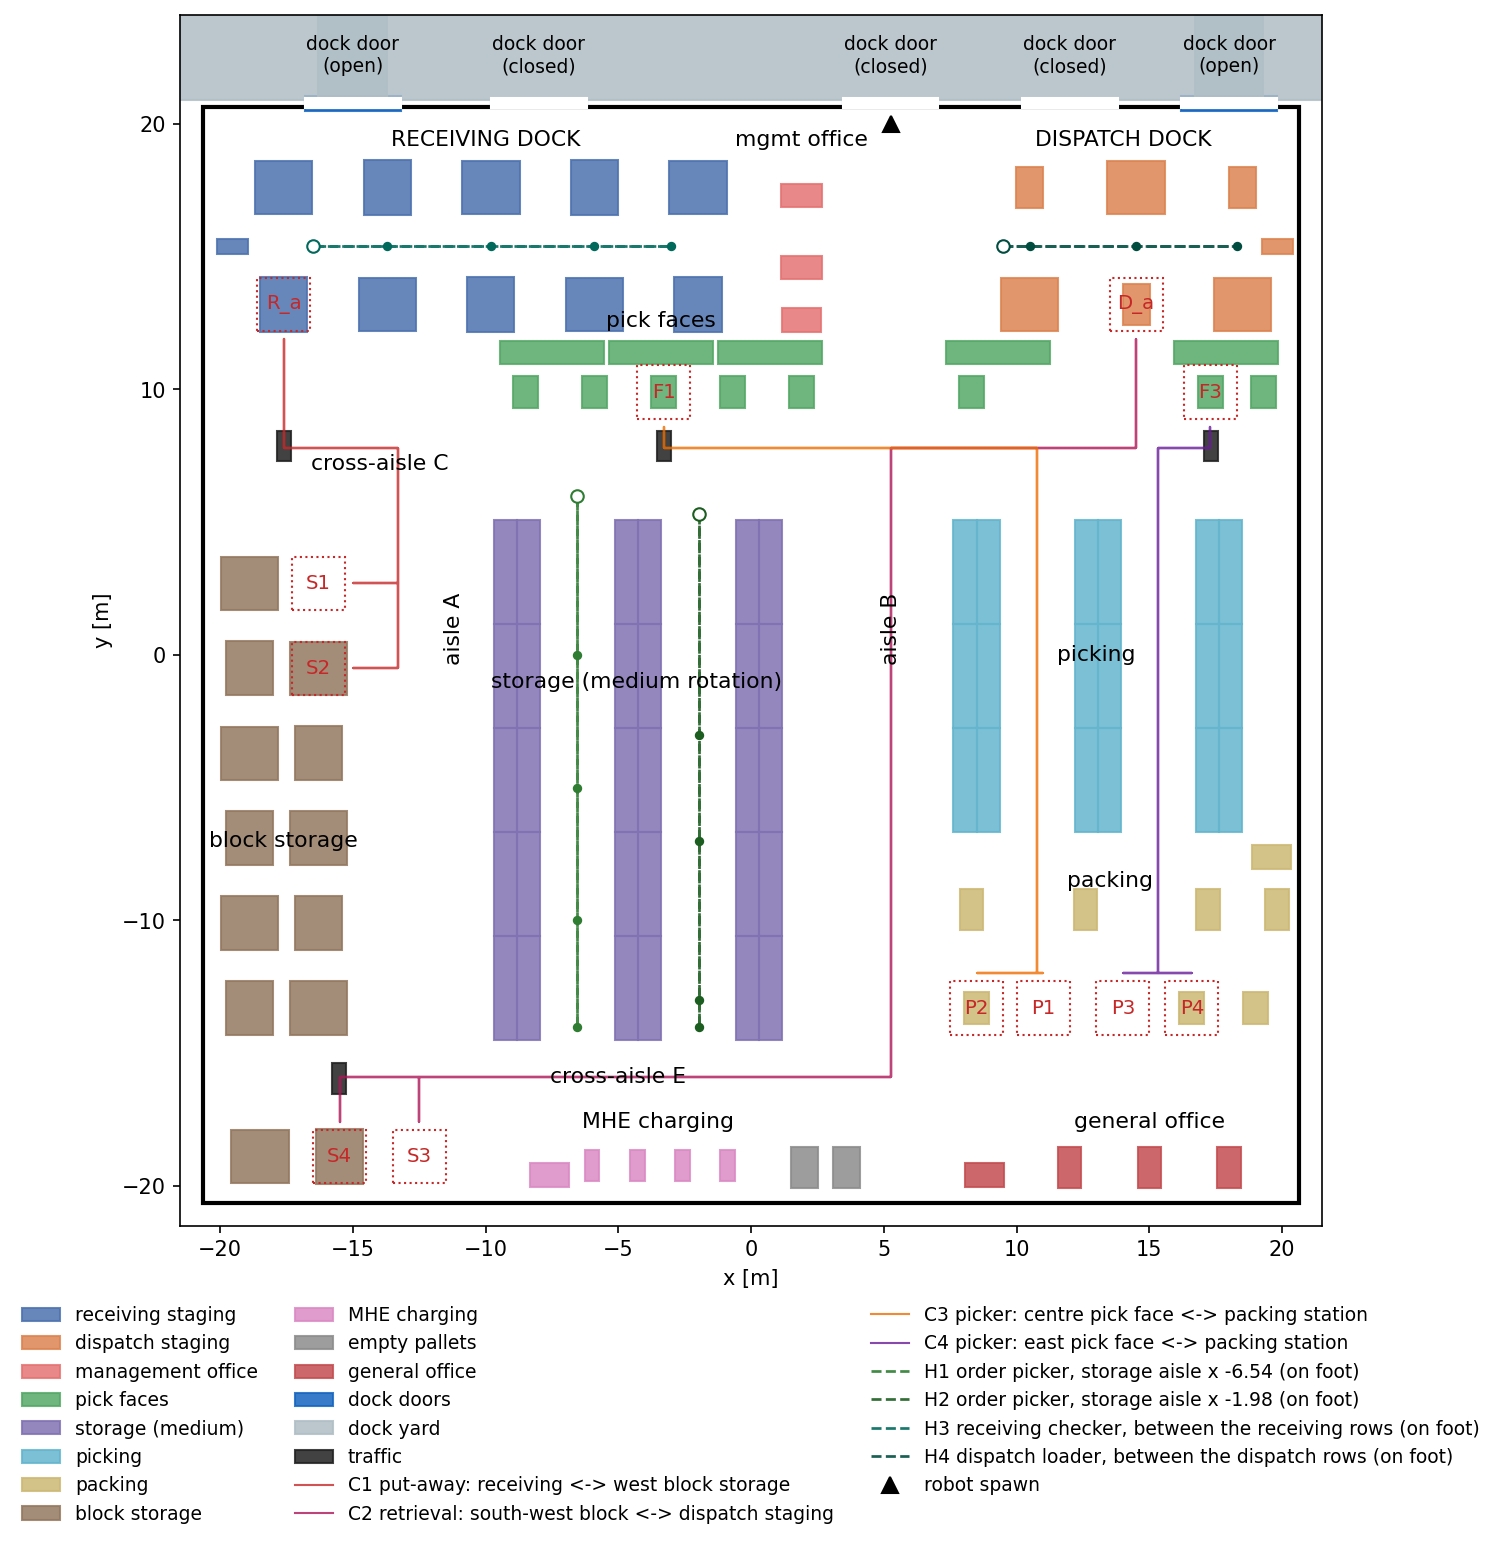
\includegraphics[width=0.92\textwidth]{figures/plan_realistic_u.png}
  \caption{Plan of the U-shape world, drawn by the generator from the tables
  that write the world file. Filled rectangles are object footprints coloured
  by zone; dotted red boxes are the exchange slots the carrier jobs pick from
  and drop on; coloured polylines are the four carrier routes; dashed green
  lines are the routes of the four people on foot, a dot at each stop and an
  open circle at the start. The band above the north
  wall is the dock yard with two docked trailers.}
  \label{fig:plan-u}
\end{figure}

\begin{figure}[p]
  \centering
  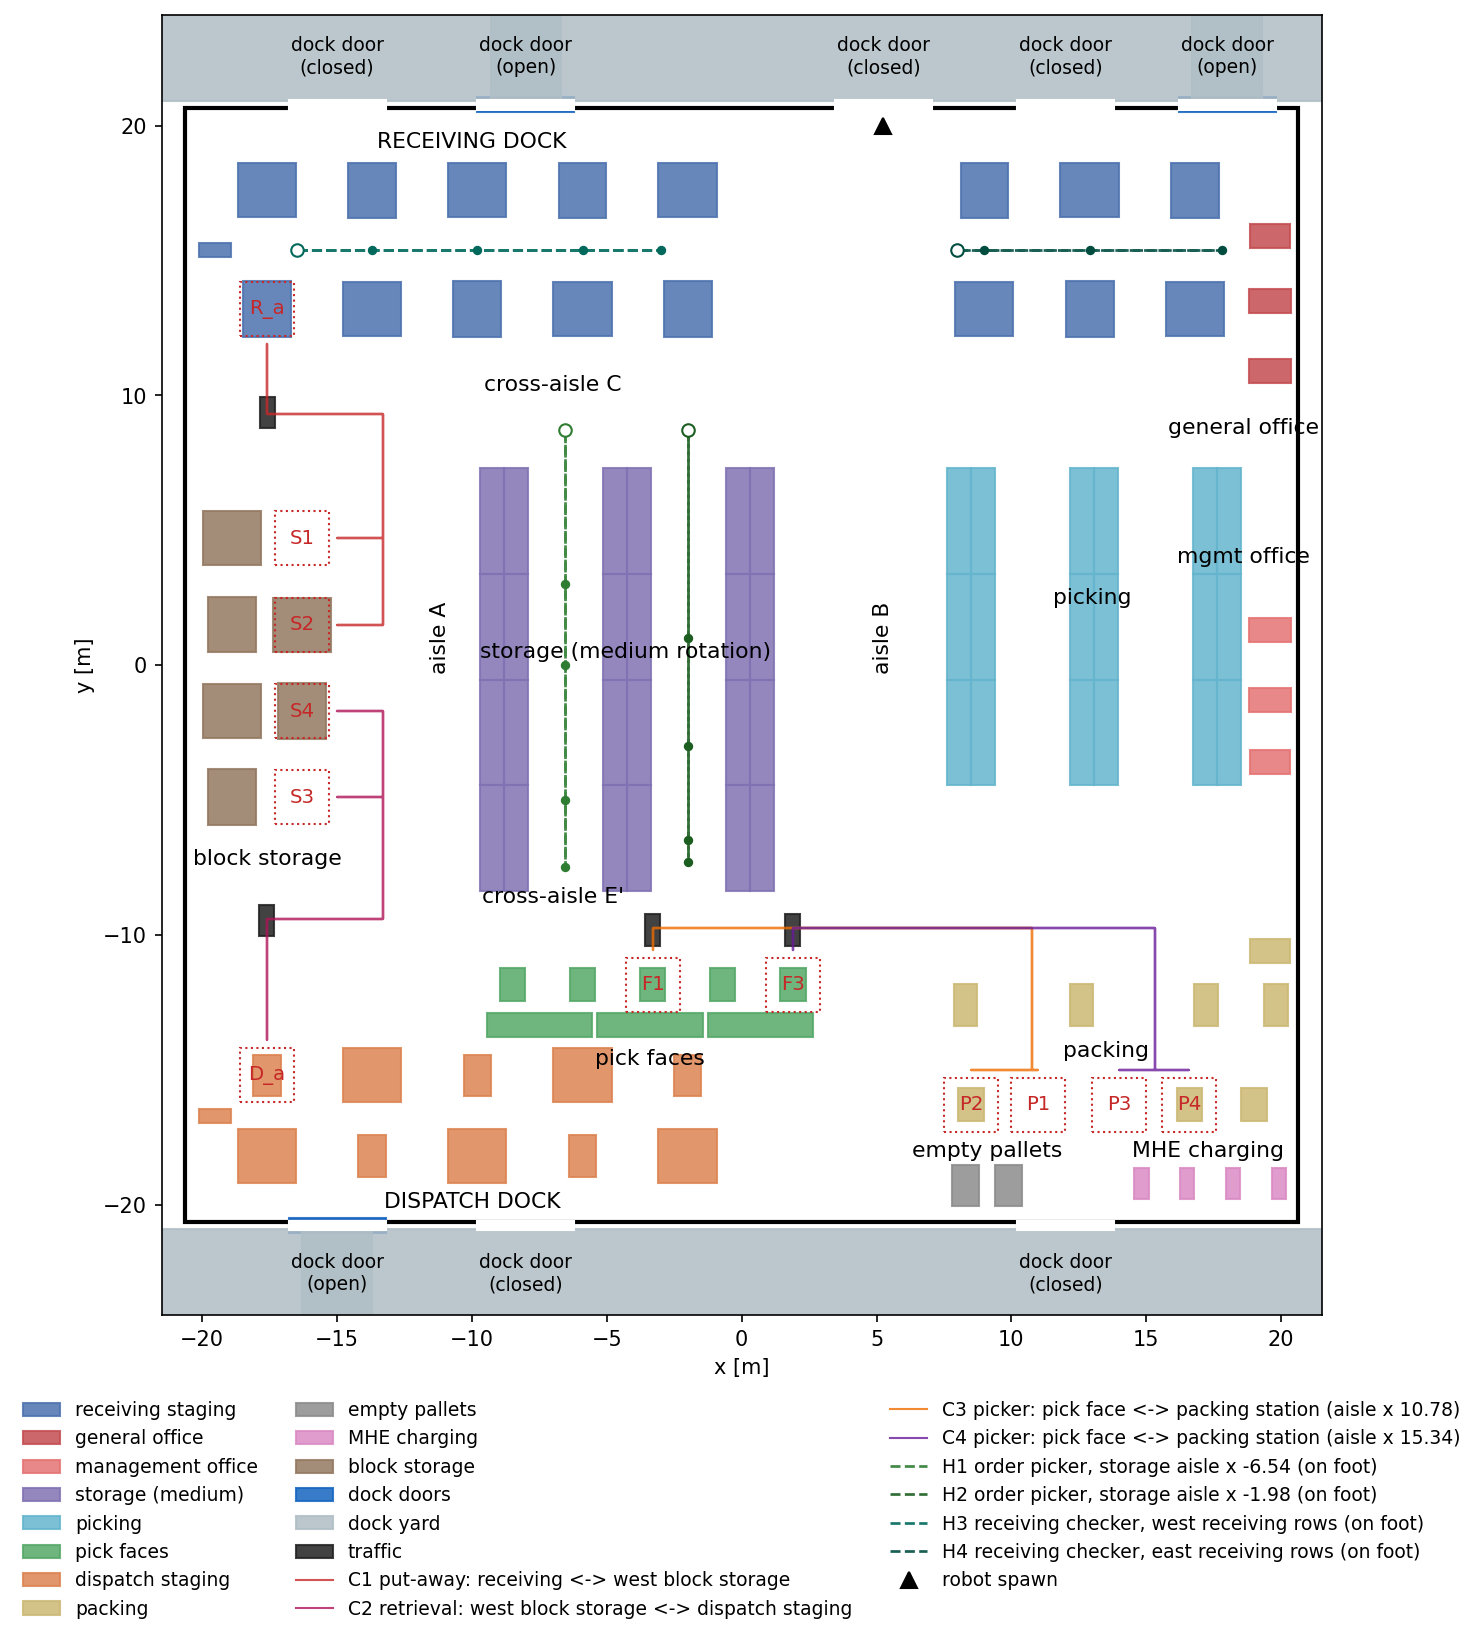
\includegraphics[width=0.88\textwidth]{figures/plan_realistic_i.png}
  \caption{Plan of the I-shape world, same conventions. Receiving docks on the
  north wall, dispatch docks on the south wall. The routes recorded before this
  layout existed do not fit it, so the I-shape recordings use a new route.}
  \label{fig:plan-i}
\end{figure}

\begin{table}[htbp]
\centering
\caption{Zones of the two worlds and the number of object instances each
holds, counted from the generator's tables. ``Inside'' excludes the dock doors,
trailers and yard. The four carriers are the pallet jacks the traffic plugin
drives; the people are actors, not objects.}
\label{tab:zones}
\small
\begin{tabularx}{\textwidth}{>{\raggedright\arraybackslash}p{0.26\textwidth}>{\raggedright\arraybackslash}Xrr}
\toprule
Zone & Contents & U-shape & I-shape \\
\midrule
Receiving staging & pallet loads in two rows, one parked jack & 11 & 17 \\
Dispatch staging & pallet loads in two rows, one parked jack & 7 & 11 \\
Pick faces & east--west shelves with totes in front & 13 & 8 \\
Storage, medium rotation & three double rack rows & 30 & 24 \\
Picking & three double rack rows & 18 & 18 \\
Packing & four desks, totes, bin & 8 & 8 \\
Block storage & floor-stacked pallets, one empty cell per job & 13 & 6 \\
Management office & two desks, bin & 3 & 3 \\
General office & desks, bin & 4 & 3 \\
MHE charging & parked pallet jacks, bin & 5 & 4 \\
Empty pallets & stacks & 2 & 2 \\
Carriers (traffic) & pallet jacks on jobs & 4 & 4 \\
People on foot (actors) & order pickers and dock checkers & 4 & 4 \\
\midrule
Inside the walls & & 118 & 108 \\
Dock doors, trailers, yard & & 8 & 13 \\
Total object instances & & 126 & 121 \\
\midrule
Baked occupancy [\si{\percent} of cells] & & 20.7 & 19.1 \\
\bottomrule
\end{tabularx}
\end{table}

\begin{figure}[htbp]
  \centering
  \begin{minipage}[t]{0.48\textwidth}
    \centering
    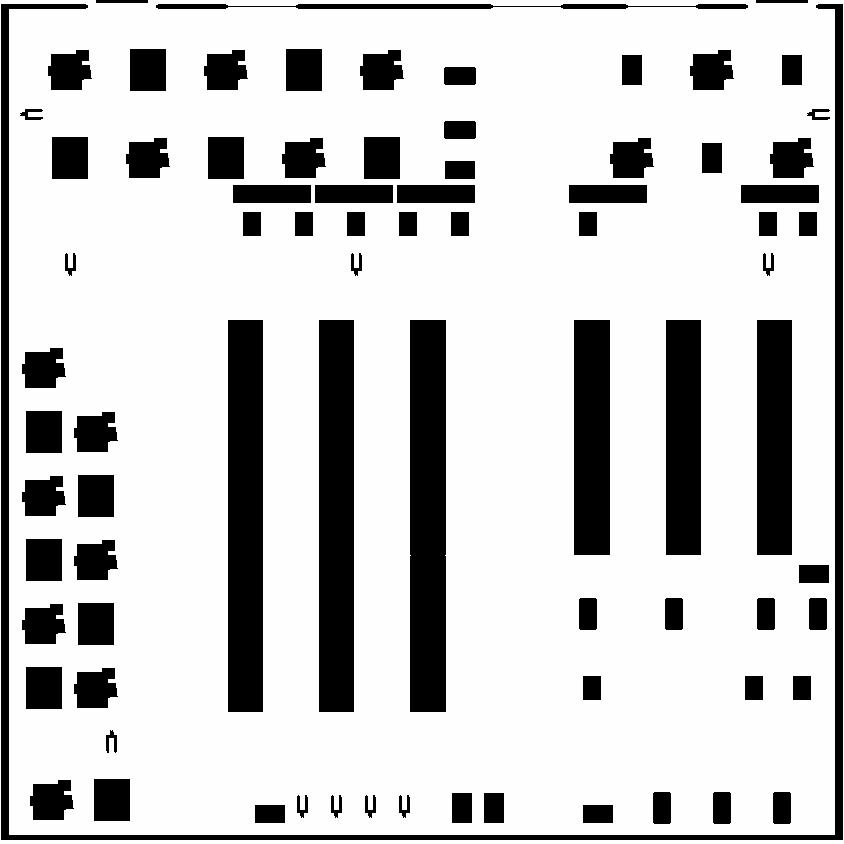
\includegraphics[width=\textwidth]{figures/warehouse_realistic_u.png}\\[0.4ex]
    {\footnotesize (a) U-shape, \SI{20.7}{\percent} occupied}
  \end{minipage}\hfill
  \begin{minipage}[t]{0.48\textwidth}
    \centering
    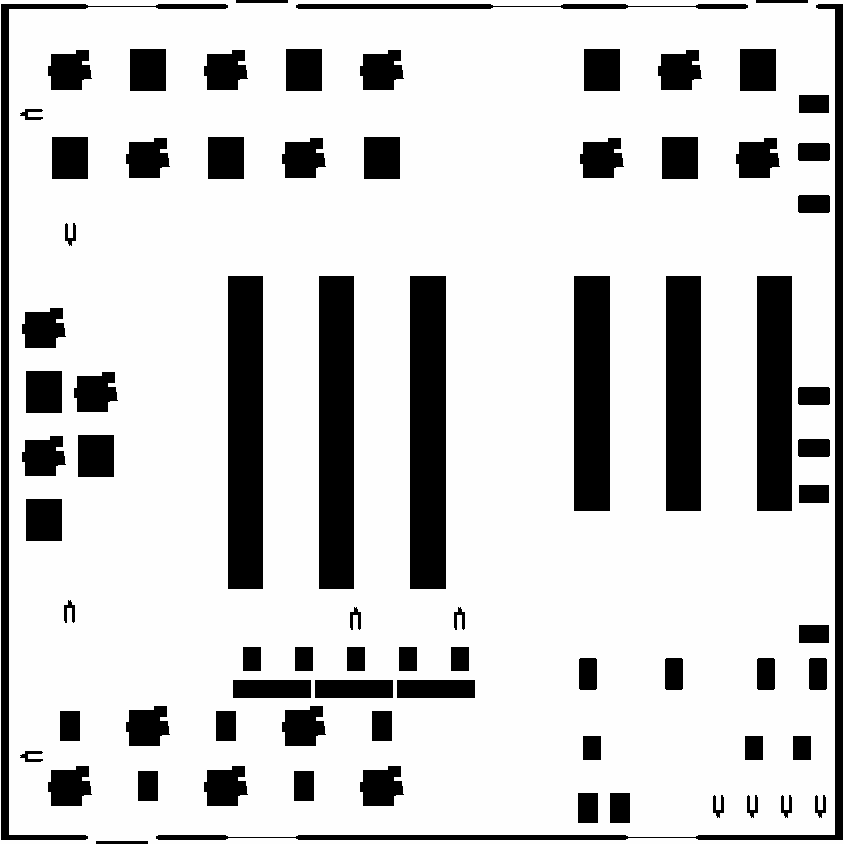
\includegraphics[width=\textwidth]{figures/warehouse_realistic_i.png}\\[0.4ex]
    {\footnotesize (b) I-shape, \SI{19.1}{\percent} occupied}
  \end{minipage}
  \caption{Baked occupancy truth of the two worlds: \SI{42.2}{\metre} square at
  \SI{0.05}{\metre} per cell, origin $(-21.1,-21.1)$~m. Carriers and loads are
  baked at their $t=0$ pose, where the static twin holds them permanently.
  Closed dock doors are the one-cell segments in the wall; open doors are the
  gaps.}
  \label{fig:baked}
\end{figure}

\FloatBarrier
\section{Traffic}

\paragraph{Carriers on jobs.} The moving objects are four pallet jacks driven
by a world-level Gazebo system, \path{gz_kinematic_trajectory/LogisticsScheduler.cc}.
A carrier drives to a load, takes it onto its forks, carries it through the
aisles, sets it down on a target slot and goes for the next: two jacks move
pallets between receiving, block storage and dispatch, two move totes between
the pick faces and the packing desks. Each job is a six-move rotation over two
loads and three slots that returns to its starting state, so it loops
indefinitely and no drop lands on an occupied slot. Carriers move at
\SIrange{1.2}{1.3}{\metre\per\second}, turn in place at
\SI{1.5}{\radian\per\second}, spend \SIrange{4}{5}{\second} on each pick or
drop, carry the load \SI{1.3}{\metre} ahead of the body, enter slots head-on
and leave in reverse. Before a world is written the generator proves it: every
static pair at least \SI{0.25}{\metre} apart, every job's slot bookkeeping
simulated, and the swept box of carrier plus load checked on every leg and
turn against every object not in its own job; the tightest clearance is
\SI{0.10}{\metre} at a packing-desk turn in each world.

\paragraph{People on foot.} Each world carries four walking people, Gazebo
actors on the stock Fuel skin with a walk clip between stops and a stand clip
at them: two order pickers, one per storage aisle, who stop at bays for six
seconds and turn at the aisle ends, and two dock checkers who walk the lane
between the staging rows. Walking speed is \SIrange{1.1}{1.2}{\metre\per\second}
with staggered starts; a \SI{0.7}{\metre} person box is swept along every leg
against the statics (at least \SI{0.25}{\metre}), the carrier corridors and
the other people, with tightest clearances of \SI{0.59}{\metre} to a static and
\SI{0.34}{\metre} to a carrier sweep. The pickers turn at the aisle mouths,
which puts them in view of a robot driving the cross-aisle.

\paragraph{What the traffic is not.} Everything moves kinematically: the
vehicles cost no physics and give no collision response, and two carriers
crossing one intersection at the same moment pass through each other. Actors
have no collision geometry, the occupancy bake does not see them, and the
static twins omit them. One limitation matters for scoring: an actor's
animated pose is computed on the rendering side and is not written back to
the entity state, so \path{/world/default/pose/info} reports every person at
its initial pose throughout a recording. Their positions can only be
reconstructed from the world file and the clock
(\path{script/people_script.py}); a detector ground truth for them is not yet
implemented, so Experiment~2 cannot score the people and Experiment~3 sees
them only as unlabelled motion.

\section{Static twins}

For each layout a static world,
\path{worlds/small_warehouse_static/small_warehouse_static_realistic_nofloortexture.world}
and its \path{..._01.world} counterpart, is derived by
\path{script/make_static_world.py}: every object is marked static and the
traffic plugin removed, nothing else changed. This is the methodological point
of the family. A realistic world and its twin share every footprint, so a
comparison between a recording in one and a recording in the other isolates
the moving vehicles. The comparison is not perfectly clean in practice: the two
recordings in a pair follow routes driven by hand, so route and traffic are not
separated on the U layout (\cref{sec:recordings}).

\section{The four recordings}
\label{sec:recordings}

Four \repo{dataset_allsensor_realistic} recordings were made between 9 and
14 October 2026, one per layout and twin, each carrying the full sensor set
(stereo images, IMU, joint states, wheel odometry, \repo{/clock},
\repo{/ground_truth/odometry} and the Gazebo pose stream). \Cref{tab:recordings}
summarises them from the bags; \cref{fig:scenes} shows each layout with its
recorded route.

\begin{table}[htbp]
\centering
\caption{The four recordings (\repo{dataset_allsensor_realistic_000} to \repo{_003}), read from the bags
(\repo{script/render_dataset_scene.py}). ``Objects'' counts obstacle instances
whose collision geometry intersects the robot-height band, excluding the wall
ring; ``Route'' is the ground-truth path length; ``Truth samples'' is the
number of ground-truth odometry messages.}
\label{tab:recordings}
\small
\begin{tabular}{lllrrrr}
\toprule
Recording & Layout & Dynamics & Objects & Route [\si{\metre}] & Sim span [\si{\second}] & Truth samples \\
\midrule
\repo{realistic_000} & U & static twin & 125 & 171.3 & 125.5 & 6278 \\
\repo{realistic_001} & I & static twin & 119 & 133.0 & 96.9 & 4847 \\
\repo{realistic_002} & U & traffic & 125 & 102.7 & 79.5 & 3975 \\
\repo{realistic_003} & I & traffic & 119 & 158.0 & 117.0 & 5852 \\
\bottomrule
\end{tabular}
\end{table}

\begin{figure}[p]
  \centering
  \begin{minipage}[t]{0.48\textwidth}\centering
    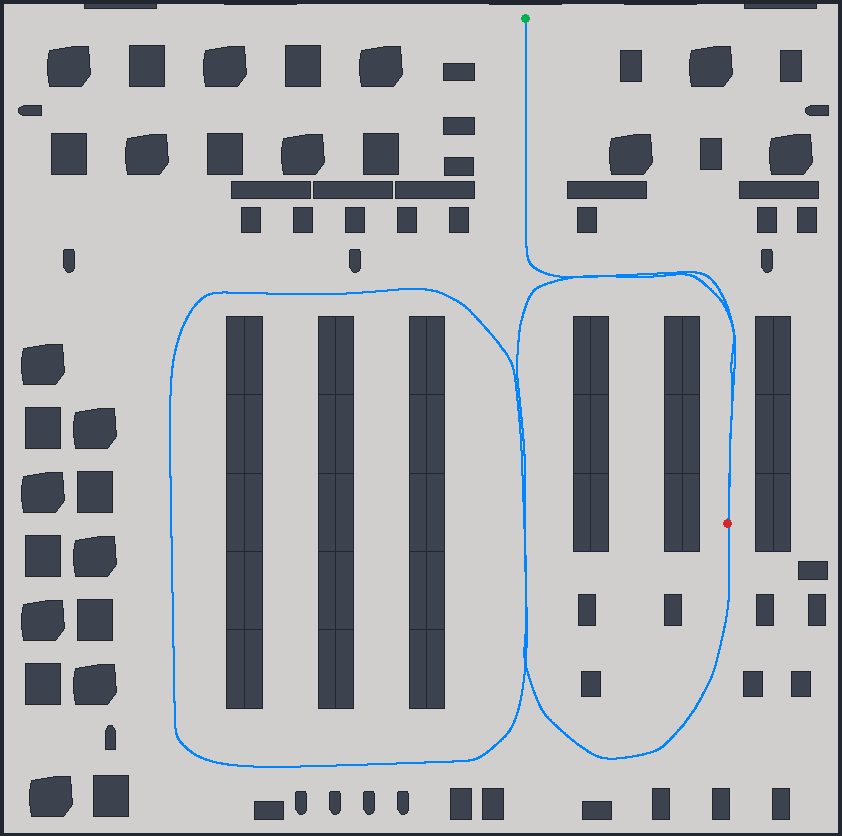
\includegraphics[width=\textwidth]{figures/scene_allsensor_realistic_000.png}\\[0.3ex]
    {\scriptsize \repo{realistic_000}: U-shape, static twin}
  \end{minipage}\hfill
  \begin{minipage}[t]{0.48\textwidth}\centering
    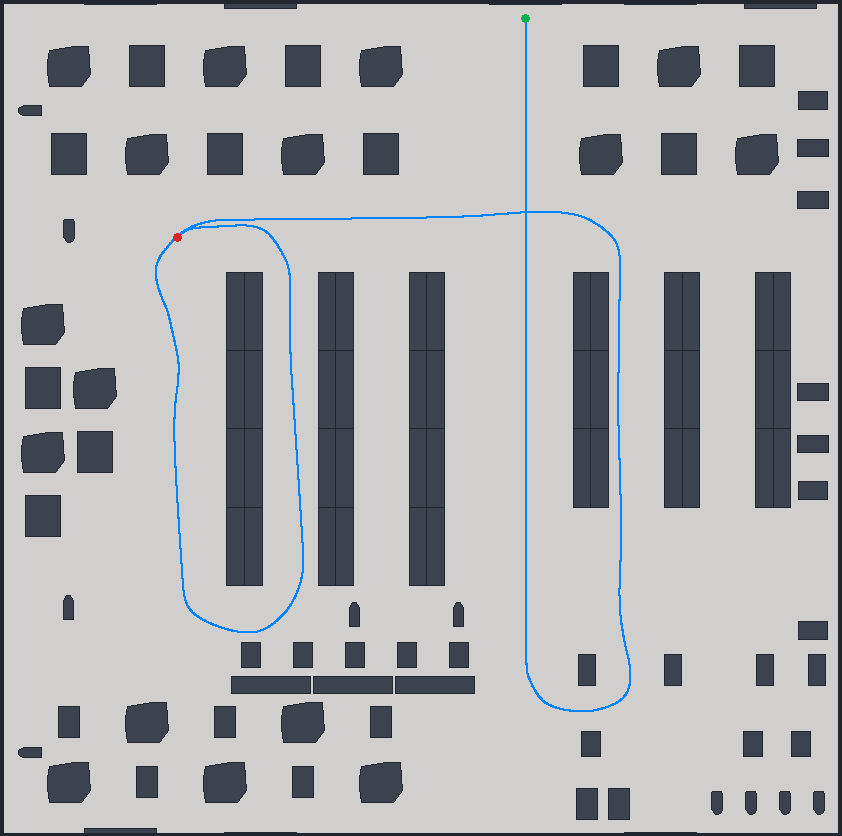
\includegraphics[width=\textwidth]{figures/scene_allsensor_realistic_001.png}\\[0.3ex]
    {\scriptsize \repo{realistic_001}: I-shape, static twin}
  \end{minipage}\\[1ex]
  \begin{minipage}[t]{0.48\textwidth}\centering
    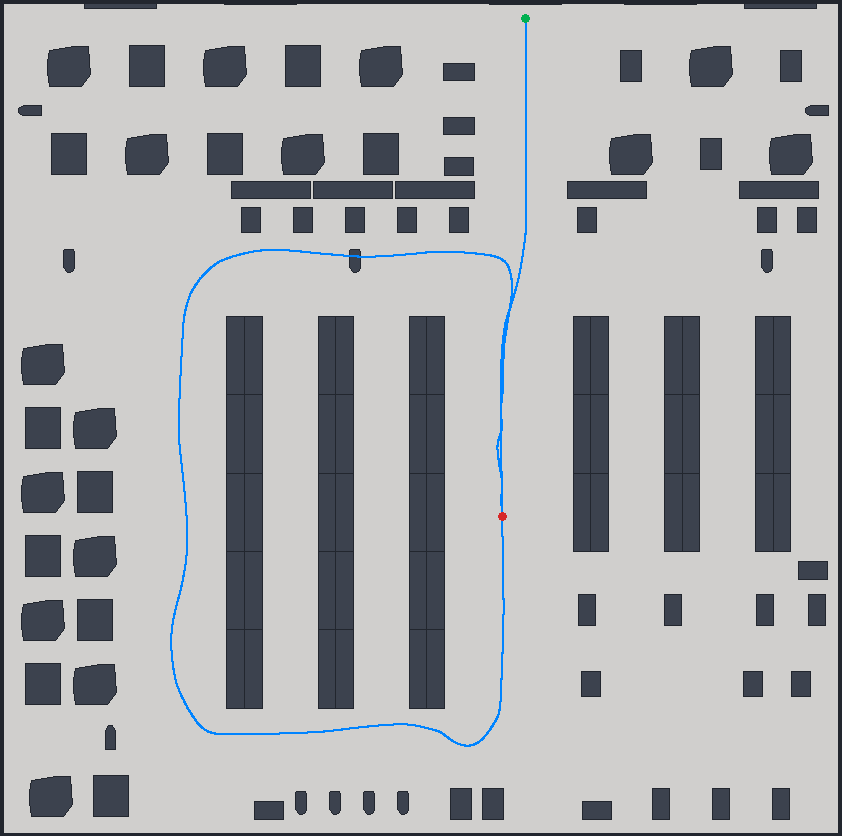
\includegraphics[width=\textwidth]{figures/scene_allsensor_realistic_002.png}\\[0.3ex]
    {\scriptsize \repo{realistic_002}: U-shape, traffic}
  \end{minipage}\hfill
  \begin{minipage}[t]{0.48\textwidth}\centering
    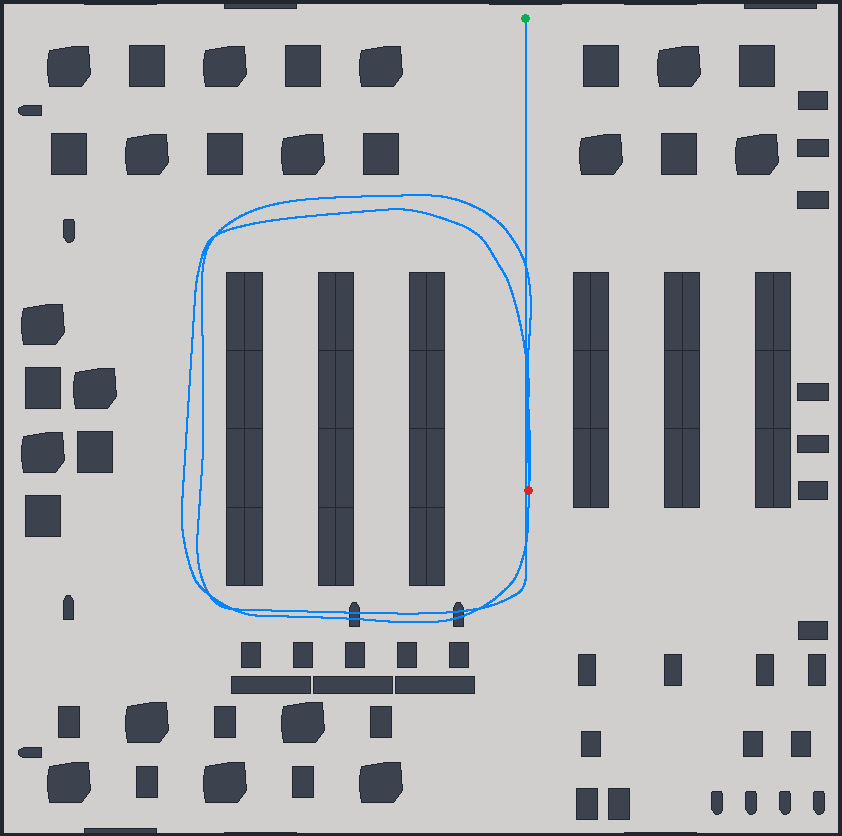
\includegraphics[width=\textwidth]{figures/scene_allsensor_realistic_003.png}\\[0.3ex]
    {\scriptsize \repo{realistic_003}: I-shape, traffic}
  \end{minipage}
  \caption{Each recording as a scene: obstacle footprints at robot height
  (convex hulls of the collision meshes), the ground-truth route in blue from
  the green start to the red end. Moving carriers are drawn at their $t=0$
  pose; the people are actors without collision geometry and do not appear.}
  \label{fig:scenes}
\end{figure}

The U-shape routes are not the same in the two U recordings. The static twin's
route is \SI{171}{\metre} over \SI{126}{\second}; the traffic recording's is
\SI{103}{\metre} over \SI{80}{\second}, so on this layout a difference between
the two recordings mixes route with traffic. The I-shape pair is closer in
length (\SI{133}{\metre} and \SI{158}{\metre}) but is also hand-driven. The
recorded routes keep to the aisles the generator reserved: on the U layout
aisles A ($x\approx-11.2$~m) and B ($x=5.25$~m, the dock lane the robot spawns
in) and cross-aisles C and E, which the original teleop route clears by at
least \SI{0.69}{\metre}; on the I layout the original route crosses the racks,
so both I recordings follow a new one.

\paragraph{Traffic actually met.} The Gazebo pose stream of the two traffic
recordings names the models that moved: on \repo{realistic_002} the four
carriers and six carried loads, on \repo{realistic_003} the four carriers and
their loads likewise; the static twins contain no moving model. From those
poses, the ground-truth heading and the shelf footprints, a carrier or load is
in the camera's view (within \SI{20}{\metre}, within $\pm\SI{45}{\degree}$,
line of sight clear) for a median \SI{37}{\percent} of the tracked time of the
traffic recordings; the people are absent from the stream and are not counted
(\path{script/extract_traffic.py}, Experiment~3 insight document).

\paragraph{The first recording of the family.} \repo{dataset_map_realistic}
(8 October 2026, \SI{126.9}{\second} simulated, \SI{151.1}{\metre} route at a
median \SI{1.38}{\metre\per\second}) preceded the four and is the only
simulation recording close to the \SI{1.5}{\metre\per\second} of the problem
statement. It was recorded without a run manifest; the bag's model inventory
identifies the U-shape world with every model stationary, which is consistent
with the static twin and with the dynamic world loaded without its traffic
plugin. It is used for mapping, not in the Experiment~3 realistic slot.

\section{Limits that apply when the recordings are scored}

\begin{itemize}
\item \textbf{Kinematic traffic.} The vehicles and people have no physics and
      no collision response; a robot driving into one passes through it. The
      visual effect on the cameras is the one being tested; the dynamic
      consequence is not simulated.
\item \textbf{People unlabelled.} Their poses are not in the bag, their
      detector truth is not implemented, and the detector weights do not
      include a person class. Every traffic statistic in Experiment~3 is a
      lower bound on the moments something moving was in the image.
\item \textbf{Route and traffic not separated.} One hand-driven recording per
      cell; on the U layout the routes differ in length by two thirds.
\item \textbf{Plain floor.} The family exists only in the
      \texttt{nofloortexture} condition; the bay-line floor of the earlier
      arrangements was not generated for it.
\item \textbf{Ground-truth reference point.} \repo{/ground_truth/odometry}
      reports the robot model origin; both visual estimators report the IMU,
      \SI{0.338}{\metre} ahead and \SI{0.192}{\metre} above it. Scoring moves
      the ground truth to the IMU point before alignment (22 October 2026); the
      scene figures draw the model-origin route.
\end{itemize}

\begin{queried}[Visual verification, carried over from Chapter 3]
The generator-side checks are complete, and the first Gazebo session on
6 October 2026 found and fixed one defect the checks could not see. Three
things remain to be confirmed by eye rather than by the checker: that loads
ride on the fork side of the jack, the shading of the generated door, trailer
and yard meshes, and the open or closed state of each door. Until then the
worlds are implemented in geometry and partial in visual verification.
\end{queried}

\section{Where the recordings are used}

The four recordings form the realistic-world half of Experiment~3
(\path{insights/experiment_3/}, Section 4.3.1 of the chapter): the unfiltered
baselines of both estimators on all four, the class and motion-masked arms on
the two traffic recordings, and the timeline and insight analyses
(\path{insights/experiment_3_insight/}). Their ground truth is extracted to
\path{output/output_vins/simulation/dataset_allsensor_realistic_00*/ground_truth.csv};
the bags themselves are held on the external drive, not in the workspace.

\end{document}
